    Jest to dowód, który najłatwiej zrozumieć samemu rozrysowując sobie proces na kartce. Niemniej, z pomocą rysunków spróbuję go Wam przybliżyć.
    
    \begin{theorem}[Vizing]
        $$\Delta(G) \leq \chi'(G) \leq \Delta(G) + 1$$
    \end{theorem}
    
    \begin{proof}
        Ograniczenie dolne widzimy od razu -- $\Delta$ krawędzi spotykających się w jednym wierzchołku musi dostać różne kolory. 
        
        Ograniczenie górne pokazujemy indukcją po liczbie pokolorowanych krawędzi. Jedną krawędź umiemy pokolorować bez problemu.
        Weźmy zatem częściowe kolorowanie i powiedzmy, że chcemy pokolorować krawędź $(x, y)$.
        
        Skoro mamy do dyspozycji $\Delta + 1$ kolorów to znaczy, że każdy wierzchołek ma jakiś kolor wolny (nie wychodzi z niego krawędź w tym kolorze). 
        
        Obserwacja, z której będziemy dużo korzystać: jeśli dowolne wierzchołki $x$, $y$ połączone krawędzią mają wolny ten sam kolor $\beta$
        to krawędź między nimi możemy pokolorować na tenże kolor. Kolory wolne dla danego wierzchołka będziemy oznaczać linią przerywaną. dotykającą tego wierzchołka.
        
        \begin{figure}[ht]
            \centering
            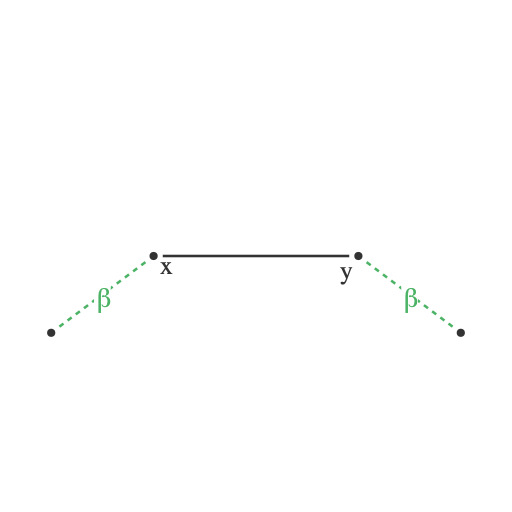
\includegraphics[scale=0.6]{chapters/dyskretna/colours/vizing/images/trivial_case.png}
            \caption{prosty przypadek; $x$ i $y$ mają wolny ten sam kolor $\beta$}
        \end{figure}
        
        Załóżmy więc, że mamy pecha i wierzchołki $x, y$ nie mają wspólnych wolnych kolorów tj. jeśli $x$ ma wolny kolor $\beta$
        to $y$ ma ten kolor zajęty i vice versa. Dodatkowo niech $\alpha_0$ będzie wolnym kolorem wierzchołka $y$.
        
        Od tego momentu będziemy tak kombinować, żeby $x$ zwolnić $\alpha_0$, być może zajmując przy tym $\beta$.
        
        \begin{figure}[H]
            \centering
            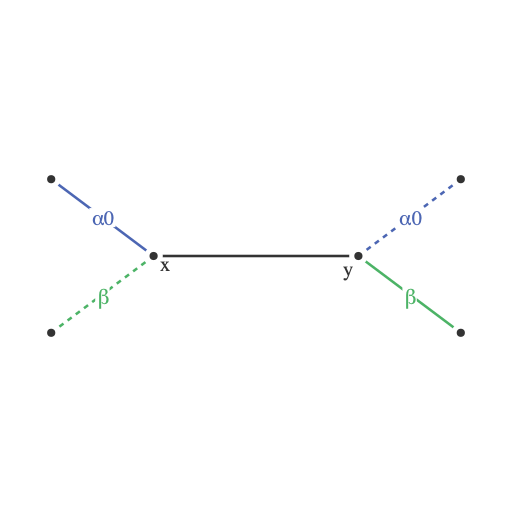
\includegraphics[scale=0.6]{chapters/dyskretna/colours/vizing/images/pre_step_one.png}
            \caption{$x$ i $y$ nie mają wspólnych wolnych kolorów}
        \end{figure}
        
        
        Niech $x_0$ będzie taki, że krawędź $(x, x_0)$ ma kolor $\alpha_0$. Jeśli $x_0$ ma wolny kolor $\beta$
        to krawędź $(x, x_0)$ możemy przekolorować na kolor $\beta$,
        tym samym sprawiając, że $x$ ma wolne $\alpha_0$.
        Ale w takiej sytuacji możemy pokolorować $(x, y)$ na kolor $\alpha_0$. 
        
        Zatem sytuacja ma się teraz tak:
        
        \begin{figure}[ht]
            \centering
            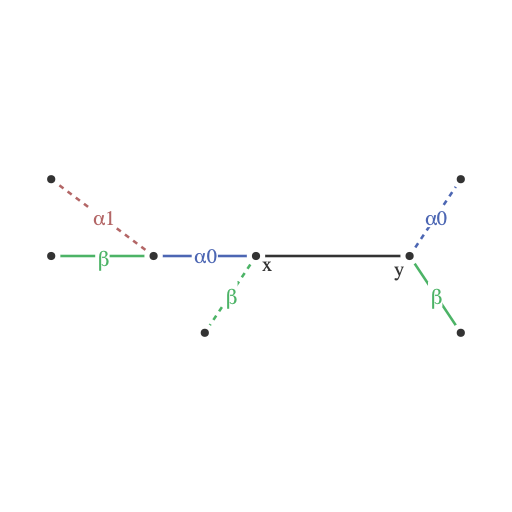
\includegraphics[scale=0.6]{chapters/dyskretna/colours/vizing/images/step_one.png}
            \caption{$x$ i $y$ mają wolne różne kolory, $x_0$ ma zajętą $\beta$ i wolne $\alpha_0$}
        \end{figure}
        
        Jeżeli teraz $x$ ma wolny kolor $\alpha_1$ to krawędź $(x, x_0)$
        możemy przekolorować na $\alpha_1$, a krawędź $(x, y)$ na $\alpha_0$. Niech więc $(x, x_1)$ będzie w kolorze $\alpha_1$.
        
        Jeśli $x_1$ miałby wolny kolor $\beta$ to możemy przekolorować $(x, x_1)$ na $\beta$, wtedy $x$ zwalnia się $\alpha_1$ a z tym wiemy co robić. 
        No to niech w $x_1$ $\beta$ będzie zajęta, a wolny będzie kolor $\alpha_2$. Poniżej ilustracja:
        
        \begin{figure}[ht]
            \centering
            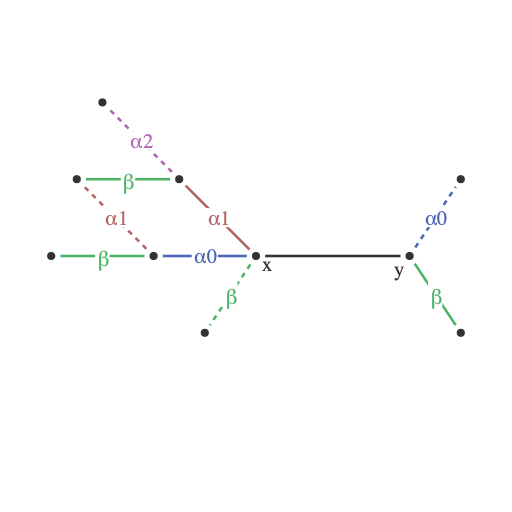
\includegraphics[scale=0.6]{chapters/dyskretna/colours/vizing/images/step_two.png}
            \caption{$x_1$ ma zajętą $\beta$ a wolne $\alpha_2$}
        \end{figure}
        
        Podobnie jak wcześniej stwierdzamy, że z $x$ wychodzi krawędź w kolorze $\alpha_2$, bo inaczej przekolorujemy $(x, x_1)$ na $\alpha_2$. Kontynuujemy to rozumowanie aż napotkamy wierzchołek $x_k$ o wolnym kolorze $\alpha_j$, który już znajduje się wśród kolorów $\alpha_0, ..., \alpha_{k-1}$
        
        
        \begin{figure}[ht]
            \centering
            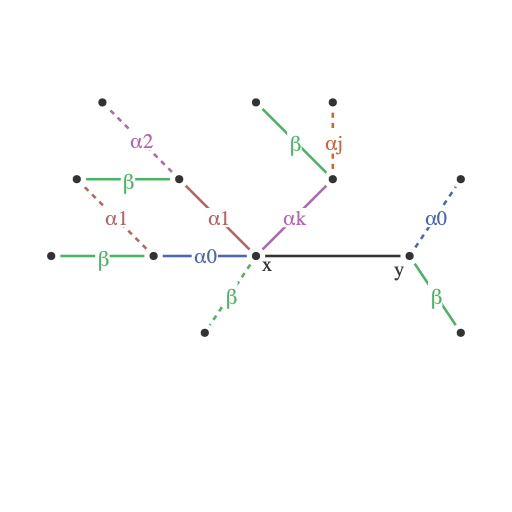
\includegraphics[scale=0.6]{chapters/dyskretna/colours/vizing/images/step_three.png}
            \caption{$x_k$ ma wolny kolor $\alpha_j$, który już widzieliśmy.}
        \end{figure}
        
        Niestety nie możemy wykonać tej samej sztuczki z przekolorowaniem co wcześniej, ale to nic nie szkodzi bo zrobimy co innego.
        Otóż wyjdźmy z wierzchołka $x_k$ i pójdźmy ścieżką w kolorach na przemian $\beta$ i $\alpha_j$.
        Oczywiście kiedyś skończą nam się krawędzie i wylądujemy w jakimś wierzchołku $v$.
        
        Rozważmy sobie teraz przypadki czym ten wierzchołek $v$ jest.
        
        \begin{enumerate}
            \item $v \notin \{x, x_0, x_1, ..., x_k\}$ 
            Najfajniejszy przypadek - ścieżka kończy się w niezbyt istotnym miejscu. Zamieniamy kolory na ścieżce miejscami. Możemy tak zrobić, bo wewnętrznym wierzchołkom się nic nie zmienia, a na końcach odpowiedni kolor jest wolny.
            
            Teraz, począwszy od krawędzi $(x, x_k)$ przekolorujemy wachlarz. 
            Dzięki przekolorowaniu, $x_k$ ma teraz wolną $\beta$ tak jak $x$, zatem $(x, x_k)$ możemy dać kolor $\beta$ 
            W takim razie $x$ ma teraz wolny kolor $\alpha_k$ tak jak $x_{k - 1}$, 
            zatem $(x, x_{k-1})$ dostanie kolor $\alpha_k$.
            Podobnie $(x, x_{k-2})$ dostanie kolor $\alpha_{k-1}$.
            
            W końcu dojdziemy do $(x, x_0)$, które dostanie kolor $\alpha_1$. Sprawiliśmy, że $x$ ma wolne $\alpha_0$,
            więc z czystym sumieniem kolorujemy $(x, y)$ na $\alpha_0$. 
            
            \begin{figure}[H]
                \centering
                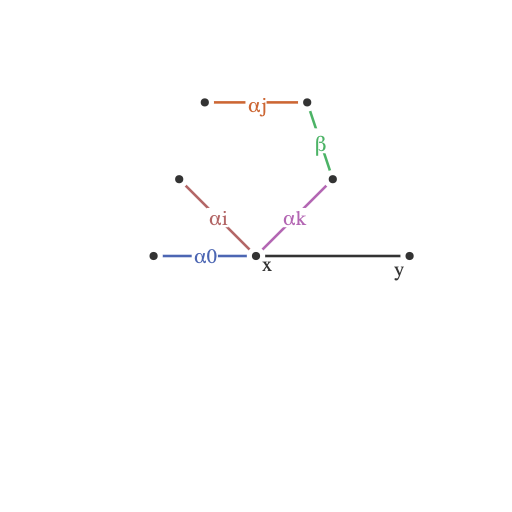
\includegraphics[scale=0.45]{chapters/dyskretna/colours/vizing/images/fan_case_one_before.png}
                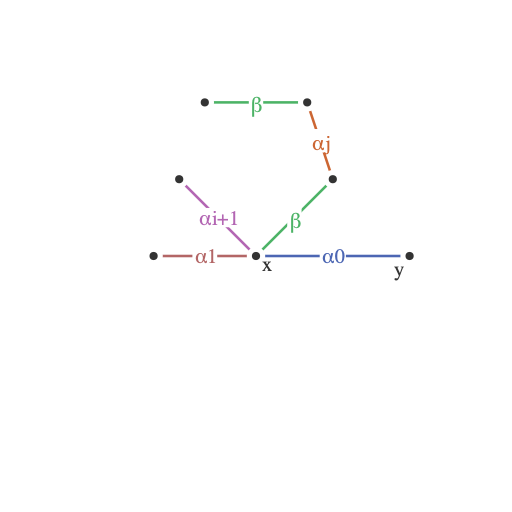
\includegraphics[scale=0.45]{chapters/dyskretna/colours/vizing/images/fan_case_one_after.png}
                \caption{Przekolorowanie wachlarza gdy ścieżka z $x_k$ kończy się w poza wierzchołkami $x, x_0, ..., x_k$}
            \end{figure}
            
            \item $v = x_{j - 1}$ 
            Taka sytuacja niestety może zajść, bo $x_{j-1}$ ma wolny kolor $x_j$ i zajętą $\beta$.
            Zauważmy, że nie możemy zrobić tego co w przypadku pierwszym, bo przekolorowanie ścieżki sprawia, że $x_{j-1}$ ma kolor $\alpha_j$ zajęty, a taki kolor by otrzymał przy poprawianiu wachlarza. Zrobimy zatem co innego.
            
            Tak jak wcześniej przekolorujemy ścieżkę,
            ale zamiast przekolorowywać krawędź $(x, x_k)$ na $\beta$
            przekolorujemy $(x, x_{j-1})$ na $\beta$. 
            Dalej możemy kontynuować tak jak poprzednio: $(x, x_{j-1})$ dostanie kolor $\alpha_{j-2}$ itd. (Musieliśmy przyjść do \(v\) krawędzią o kolorze \(\beta\) bo inaczej nie byłby to koniec ścieżki)
            
            
            \begin{figure}[H]
                \centering
                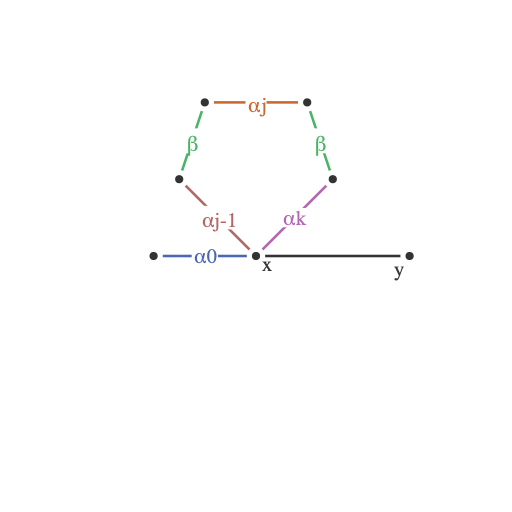
\includegraphics[scale=0.45]{chapters/dyskretna/colours/vizing/images/fan_case_three_before.png}
                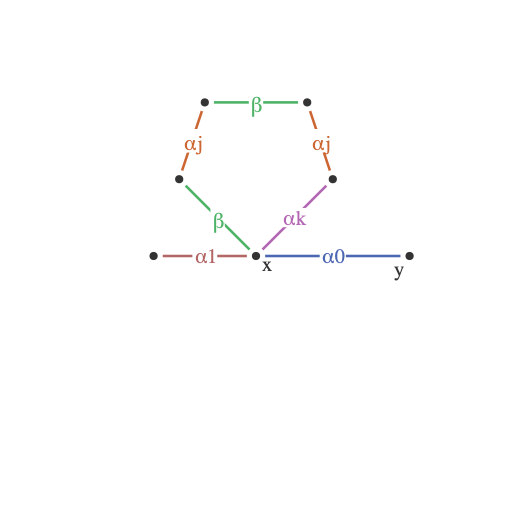
\includegraphics[scale=0.45]{chapters/dyskretna/colours/vizing/images/fan_case_three_after.png}
                \caption{Przekolorowanie gdy ścieżka z $x_k$ kończy się w $x_{j-1}$}
            \end{figure}
            
        \end{enumerate}
        
        
        
    \end{proof}